\chapter{无人机编队的动力学模型的建立}
\label{chap:formation_dynamic_equ}
本章基于无人机编队的领从方法(leader-follower method)建立无人机编队的相对运动方程。为了与无人机的解耦控制方法相匹配,本文的
模型建立将无人机运动分为水平平面运动以及竖直平面运动内分别建立数学模型。由于无人机尺寸小,强度大,飞行包线较小,现做如下假设:
\begin{itemize}
    \item 无人机为具有6自由度的三维空间运动刚体。
    \item 忽略地球自转,将地球作为惯性系。
    \item 忽略地球曲率,即所谓的“平板地球假设”。%TODO:考虑是否要加入大气的假设,以及引用文献
\end{itemize}
本章中涉及的坐标系有:
\begin{enumerate}
    \item 地面坐标系$O_gx_gy_gz_g$:$O_g$选为无人机解锁时的位置,$O_gx_g$轴指向北,$O_gy_g$轴指向东,$O_gz_g$轴符合右手定则,指向下。
    \item 导航坐标系$NED(north-east-down)$:原点选做飞机质心,$N$轴指向北,$E$轴指向东,$D$轴符合右手定则,指向下。
    \item 航迹坐标系$O_kx_ky_kz_k$:$O_k$选为无人机质心,$O_kx_k$轴始终与无人机地速方向一致,$O_kz_k$轴位于包含$O_kx_k$轴的铅垂平面内,
    $o_ky_k$符合右手定则,指向右。
    \item 机体坐标系$O_bx_by_bz_b$:$O_b$选为无人机质心,$O_bx_b$位于无人机的对称平面内,平行于机身轴线或者机翼的平均气动弦线,指向前;$O_bz_b$亦在对称平面之内,
    垂直于$O_bx_b$轴,指向下;$O_by_b$垂直于对称平面,指向右。机体坐标系始终与无人机固连。
    \item 气流坐标系$O_ax_ay_az_a$:气流坐标系又被称作风坐标系或者速度坐标系;$O_a$取作无人机质心,$O_ax_a$始终指向无人机的空速方向;$O_az_a$位于无人机对称面之内,
    垂直于$O_ax_a$轴,指向下;$O_ay_a$轴垂直于$O_ax_az_a$平面,指向右。只有在大气风速$V_{wind}=0$时,航迹系的$O_kx_k$才与气流坐标系的$O_ax_a$重合。
\end{enumerate}

本章中领机与从机的各运动学量以及几何关系分别用上标$l,f$标记,从机期望值以$“des”$上标标记;
运动学量以及几何关系所属坐标系关系则用各个坐标系的字母作为下标标记。
领机、从机在水平以及竖直平面内的几何关系分别在图\ref{fig:c02-2d_level_motion}和图\ref{fig:c02-2d_vert_motion}给出;
\begin{figure}[H]
    \centering
    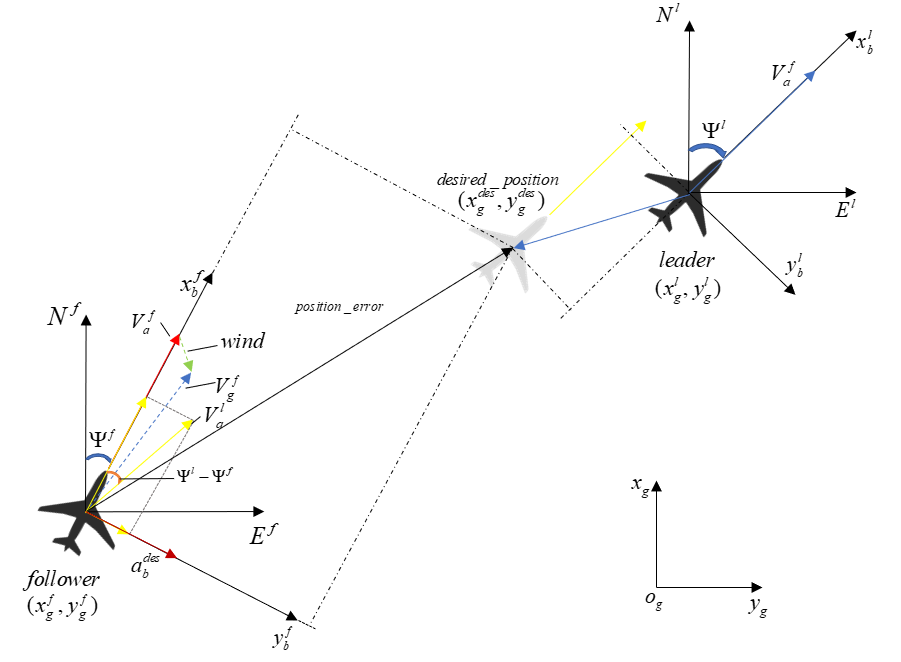
\includegraphics[width=0.75\textwidth]{figures/c2/2d_level_motion.png}
    \caption{水平平面双机编队几何关系}\label{fig:c02-2d_level_motion}
\end{figure}
\begin{figure}[H]
    \centering
    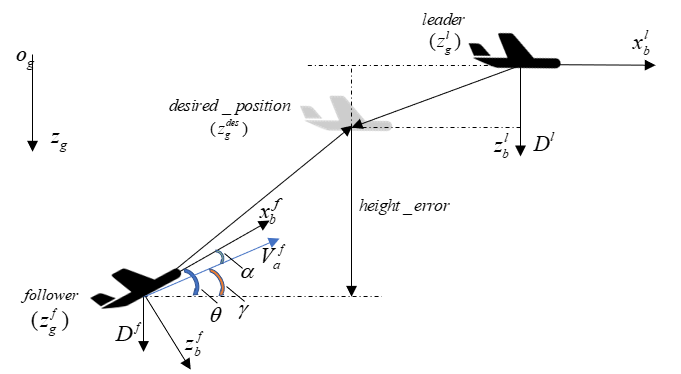
\includegraphics[width=0.75\textwidth]{figures/c2/2d_vert_motion.png}
    \caption{竖直平面双机编队几何关系}\label{fig:c02-2d_vert_motion}
\end{figure}
在图\ref{fig:c02-2d_level_motion}中:
$(x_{g}^l,y_{g}^l),(x_{g}^f,y_{g}^f),(x_{g}^{des},y_{g}^{des})$分别为领机、从机以及从机期望编队位置在地面坐标系$O_gx_gy_g$平面之中的分量;
$\Psi^l,\Psi^f$分别为领机与从机的偏航角(yaw angle);
$\chi^l,\chi^f$分别为领机与从机的航迹偏角(航迹方位角);
$V_a,V_{wind},V_g$分别为领机和从机的空速、风速以及地速向量;
$a_{b}^{des}$是从机产生的,在体轴系下的期望的法向加速度。

在图\ref{fig:c02-2d_vert_motion}中:
$z_{g}^l,,z_{g}^f,z_{g}^{des}$分别为领机、从机以及从机期望编队位置在地面坐标系$O_gz_g$轴上的分量;
$\theta^l,\theta^f$分别为领机与从机的俯仰角(pitch angle);
$\gamma^l,\gamma^f$分别为领机与从机的航迹倾角(航迹倾斜角);
$V_a,V_{wind},V_g$分别为领机和从机的空速、风速以及地速向量;
